% This file was created with tikzplotlib v0.9.17.
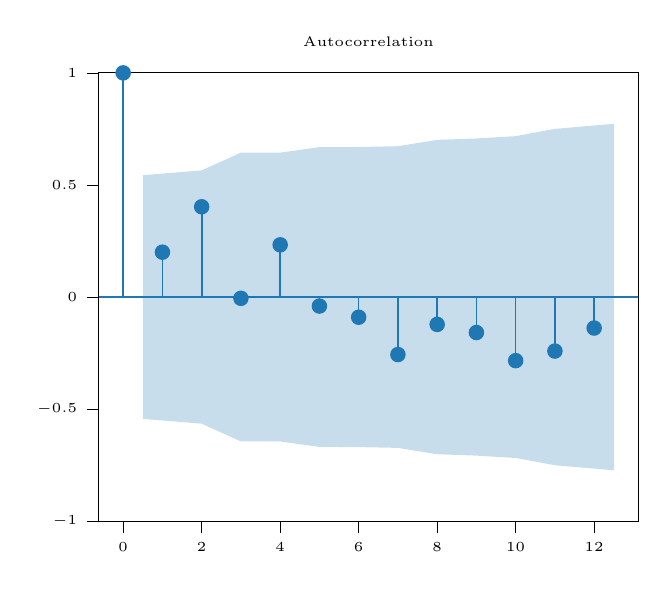
\begin{tikzpicture}

\definecolor{color0}{rgb}{0.12156862745098,0.466666666666667,0.705882352941177}

\begin{axis}[
font={\fontsize{3}{12}\selectfont},
tick align=outside,
tick pos=left,
title={Autocorrelation},
x grid style={white!69.0196078431373!black},
xmin=-0.625, xmax=13.125,
xtick style={color=black},
y grid style={white!69.0196078431373!black},
ymin=-1, ymax=1,
ytick style={color=black}
]
\path [fill=color0, fill opacity=0.25]
(axis cs:0.5,0.543596203409375)
--(axis cs:0.5,-0.543596203409375)
--(axis cs:2,-0.564944358691729)
--(axis cs:3,-0.644189697014584)
--(axis cs:4,-0.644204240871152)
--(axis cs:5,-0.66862199175734)
--(axis cs:6,-0.66933545636468)
--(axis cs:7,-0.672904705335104)
--(axis cs:8,-0.701205081289013)
--(axis cs:9,-0.707456535037507)
--(axis cs:10,-0.717846296283477)
--(axis cs:11,-0.750256944575949)
--(axis cs:12.5,-0.772786673920178)
--(axis cs:12.5,0.772786673920178)
--(axis cs:12.5,0.772786673920178)
--(axis cs:11,0.750256944575949)
--(axis cs:10,0.717846296283477)
--(axis cs:9,0.707456535037507)
--(axis cs:8,0.701205081289013)
--(axis cs:7,0.672904705335104)
--(axis cs:6,0.66933545636468)
--(axis cs:5,0.66862199175734)
--(axis cs:4,0.644204240871152)
--(axis cs:3,0.644189697014584)
--(axis cs:2,0.564944358691729)
--(axis cs:0.5,0.543596203409375)
--cycle;

\path [draw=color0, semithick]
(axis cs:0,0)
--(axis cs:0,1);

\path [draw=color0, semithick]
(axis cs:1,0)
--(axis cs:1,0.200108049246219);

\path [draw=color0, semithick]
(axis cs:2,0)
--(axis cs:2,0.402654610225704);

\path [draw=color0, semithick]
(axis cs:3,0)
--(axis cs:3,-0.00563083388067813);

\path [draw=color0, semithick]
(axis cs:4,0)
--(axis cs:4,0.232897614225945);

\path [draw=color0, semithick]
(axis cs:5,0)
--(axis cs:5,-0.0401898101890896);

\path [draw=color0, semithick]
(axis cs:6,0)
--(axis cs:6,-0.0900351564259988);

\path [draw=color0, semithick]
(axis cs:7,0)
--(axis cs:7,-0.256516559362992);

\path [draw=color0, semithick]
(axis cs:8,0)
--(axis cs:8,-0.122068171443564);

\path [draw=color0, semithick]
(axis cs:9,0)
--(axis cs:9,-0.158294179132346);

\path [draw=color0, semithick]
(axis cs:10,0)
--(axis cs:10,-0.283746651443675);

\path [draw=color0, semithick]
(axis cs:11,0)
--(axis cs:11,-0.24095877418934);

\path [draw=color0, semithick]
(axis cs:12,0)
--(axis cs:12,-0.138220137630186);

\addplot [semithick, color0]
table {%
-0.625 -2.22044604925031e-16
13.125 -2.22044604925031e-16
};
\addplot [semithick, color0, mark=*, mark size=2.5, mark options={solid}, only marks]
table {%
0 1
1 0.200108049246219
2 0.402654610225704
3 -0.00563083388067813
4 0.232897614225945
5 -0.0401898101890896
6 -0.0900351564259988
7 -0.256516559362992
8 -0.122068171443564
9 -0.158294179132346
10 -0.283746651443675
11 -0.24095877418934
12 -0.138220137630186
};
\end{axis}

\end{tikzpicture}
